\section{Montag}

\subsection{Lehrinhalte FOPT1 und FOPT2}

\subsubsection{Notizen zu den Lehrinhalten FOPT1 und FOPT2}
    \begin{itemize}
        \item Wichtige Begriffe:
        \begin{itemize}
                  \item Parallelität und Nebenläufigkeit
                  \item Prozess, Thread, Programm, Rechner, Betriebssystem, verteiltes System
        \end{itemize}
        \item Erzeugung und Start von Threads:
        \begin{itemize}
            \item Ableitung einer Klasse aus Thread und Überschreiben der Methode run
            \item Implementierung der Schnittstelle Runnable (funktionale Schnittstelle, Lambda-Ausdruck möglich)
        \end{itemize}
        \item Probleme beim Zugriff auf gemeinsame Daten:
        \begin{itemize}
            \item nicht zielführende Ansätze zur Lösung der Problematik
        \end{itemize}

        \item \textbf{Synchronized und Volatile:}
        \begin{itemize}
            \item Synchronized-Methode und -Blöcke
            \item volatile
            \item Regel für die korrekte Synchronisation
            \item[] (Damit ist die Regel gemeint, die besagt, dass, wenn mehrere Threads lesend auf Daten eines Objektes zugreifen, und mindestens ein Thread diese Daten verändert, dann muss synchronisiert werden - also die lesenden und schreibenden Zugriffe.)
        \end{itemize}

        \item \textbf{Ende von Java-Threads:}
        \item[] (main Thread endet, wenn die main-Methode zu Ende ist, Threads i.d.R., wenn ihre run-Methode zu Ende ist)
        \begin{itemize}
            \item Join, isAlive
            \item[] (join ist blockierend, der Aufrufer wartet so lange, bis der Thread beendet ist.)
            \item Statt hartem Abbrechen Programmieren des ``freiwilligen Beendens``
            \item Interrupt, isInterrupted
            \item[] (man kann eigenes Flag programmieren, das man abfragt, ob abgebrochen werden soll. Das interrupt-Flag hat den Vorteil, dass blockierende Methoden wie \code{sleep} oder \code{join} durch eine Ausnahme unterbrochen werden.)
        \end{itemize}

        \item Ende von Java-Threads:
        \begin{itemize}
            \item join, isAlive
            \item statt hartem Abbrechen Programmieren des ``freiwilligen Beendens``
            \item interrupt, isInterrupted
        \end{itemize}
        \item wait / notify / notifyAll

        \item \textbf{Semaphore:}
        \begin{itemize}
            \item Varianten: additive Semaphore und Semaphorgruppen
            \item[] (Semaphore dienen zur Synchronisation von parallelen Threads und zum gegenseitigen Ausschluss oder zu Herstellung einer vorgegebenen Ausführungsreihenfolge.
            Eine Variante davon sind \textit{Additive Semaphore}, bei denen der Zähler auf einen Schlag um mehr als 1 erhöht oder erniedrigt werden kann.)
            \item Mit und ohne Fairness
        \end{itemize}

        \item \textbf{Message Queues / Pipes}
        \item[] (Message Queues und Pipes sind Lösungen für das Erzeuger-Verbraucher-Problem mit mehr als einem Pufferplatz. Message Queues halten die Bytefolgen in der Reihenfolge vor, wie sie abgelegt wurden - man empfängt die Bytefolgen so, wie sie gesendet wurde. Bei Pipes sind die Nachrichtengrenzen nicht erkennbar, man empfängt einen Teil der gesendeten Bytes, oder mehrere Bytefolgen. )

        \item Philosophenproblem

        \item \textbf{Leser-Schreiber-Problem}
        \item[] (s. Abchnitt~\ref{subsec:readerwriterproblem} für Strategien)

        \item \textbf{Schablonen für Synchronized-Methoden:}
        \begin{itemize}
            \item Lesend mit / ohne Wait
            \item Schreibend mit / ohne Wait, mit / ohne Notify bzw. NotifyAll
        \end{itemize}

        \item \textbf{Concurrent-Klassenbibliothek:}
        \begin{itemize}
            \item Thread-Pools
            \item Locks und Conditions
            \item[](s. Abschnitt~\ref{subsubsec:locksconditions})
            \item Atomic-Klassen
            \item Synchronisationsklassen: Semaphore, CountDownLatch, CyclicBarrier, Exchanger
            \item Queue-Klassen
            \item Fork-Join-Framework
            \item[] (erweitert das Konzept von Thread-Pools für baumartige Berechnungen über \code{ForkJoinPool}; die Klasse realisiert einen Thread-Pool, die für jeden Knoten eines Berechnungsbaums einen Thread erstellt - es können dadurch von Threads neue Threads in den Pool geworfen werden. Der Nachteil bei den Thread-Pools ist, das ein Thread, der für eine Berechnung ein Ergebnis eines anderen Threads benötigt, diesen Thread über einen herkömmlichen Thread-Pool nicht selber anstoßen kann, weil neue Threads erst abgearbeitet werden können, wenn im Pool Platz für neue Aufträge da ist - wenn nun ein Thread auf einen anderen Thread wartet, hat man quasi eine Verklemmung).
            Alle Threads eines \code{ForkJoinPool}s sind Daemon Threads.
        \end{itemize}

        \item \textbf{Verklemmungen (Deadlocks):}
        \begin{itemize}
            \item Beispiele für Verklemmungen
            \item Bedingungen für das Vorliegen einer Verklemmung
            \item[] (Verklemmung entsteht, wenn es einen Zyklus von Threads gibt, so dass ein Thread auf ein Betriebsmittel wartet, welches der im Zyklus nachfolgende Thread besitzt. Betriebsmittel können z.B. passive Objekte sein. Voraussetzung ist, dass Betriebsmittel nur unter gegenseitigem Ausschluss benutzbar sind, einem Thread nicht entzogen werden können und dass Threads bereits Betriebsmittel besitzen und weitere anfordern.)
            \item Vermeidung:
            \begin{itemize}
                \item Anforderung ``auf einen Schlag``
                \item Anforderung in festgelegter Reihenfolge
                \item[] (Bsp.: Alle Philosophen bis auf einen fordern zuerst linke, dann rechte Gabel an.)
                \item Weitere Verfahren: Wound-Wait- und Wait-Die-Verfahren, Bankier-Algorithmus
            \end{itemize}
        \end{itemize}

    \end{itemize}

\subsection{Ergänzungen}
\begin{tcolorbox}
    Das ausschlaggebende Kriterium für die Verwendung von \code{notify()} / \code{notifyAll()} ist nicht die Anzahl der wartenden Threads in den Warteschlangen eines passiven Objektes, sondern ob es mehrere Threads gibt die aufgrund einer Zustandsänderung des Objektes ihre \textit{while-wait-Schleife} verlassen können (s. a. Abbildung~\ref{fig:notifynotifyall}).
\end{tcolorbox}

\begin{figure}
    \centering
    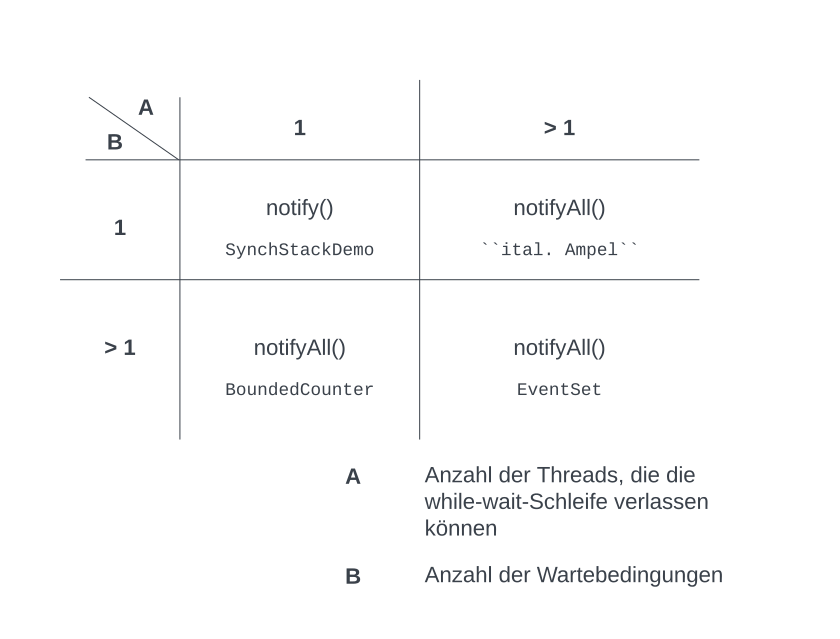
\includegraphics[scale=0.5]{chapters/Anhang/Präsenzphase/img/notifynotifyall}
    \caption{Merkregel für die Verwendung von notify()/notifyAll() mit den besprochenen Aufgaben als Beispiel. I.d.R. wird notify() nur genutzt, wenn es nur einen Thread gibt, der die while-wait-Schleife verlassen kann, und es gleichzeitig nur eine Wartebedingung für einen oder mehrere Threads gibt. (Quelle: eigene)}
    \label{fig:notifynotifyall}
\end{figure}


\subsection*{Lösung für das leser-Schreiber-Problem}

Für das Leser-Schreiber-Problem gibt es eine Methode, die einen Wächter enthält.
Der Wächter entscheidet, ob ankommende Threads in die Warteschlange geschickt werden oder aus der Warteschlange in den lesenden/schreiben Bereich gelassen werden dürfen.\\

\noindent
Wichtig ist die korrekte Beachtung der Wartebedingungen bei den unterschiedlichen Lösungsmöglichkeiten.\\

\noindent
Im Folgenden ein Beispiel für eine Lösung mit einer Warteschlange für die eintreffenden Aufgaben, es wird also jeweils der erste Eintrag aus einer Liste entfernt, falls der Eintrag in \code{doRead()} einem Leser entspricht, in \code{doWrite()} einem Schreiber.\\
In der \code{doRead()} wird darüberhinaus noch ein erneutes \code{notifyAll()} aufgerufen, um weitere \textbf{Leser} aus der Warteschlange zu holen - gleichzeitiger Zugriff mehrerer Leser ist ja erlaubt.\\
Hingegen ist die Wartebedingung in der \code{doWrite()} dergestalt, dass nur geschrieben werden darf, wenn es sonst
\begin{itemize}
    \item keinen aktiven Leser gibt
    \item keinen aktiven Schreiber gibt (es darf immer nur \textit{ein} Schreiber gleichzeitig aktiv sein)
\end{itemize}



\noindent
\begin{minted}[mathescape,
    linenos,
    numbersep=5pt,
    gobble=2,
    fontsize=\small,
    frame=lines,
    framesep=2mm]{java}
    class Book {

        public function read() {
            canRead();
            try {
                doRead();
            } finally {
                endRead();
            }
        }

        public function write() {
            canWrite();
            try {
                doWrite();
            } finally {
                endWrite();
            }
        }

        private synchronized void canWrite() {
            queue.add(Thread.currentThread());

            // only write if there is no reader, no other writer
            // and the first in queue is a writer
            while (!(queue.get(0) instanceof Writer) ||
                    activeReaders > 0 || activeWriters > 0) {
                try {
                    this.wait();
                } catch (InterruptedException e) {

                }
            }
            activeWriters++;
            queue.removeFirst();
        }

        private synchronized void canRead() {
            queue.add(Thread.currentThread());
            // read if first in queue is reader and no writer is active
            while (!(queue.get(0) instanceof Reader) || activeWriters > 0) {
                try {
                    this.wait();
                } catch (InterruptedException e) {

                }
            }
            activeReaders++;
            queue.removeFirst();
            // notifyAll() to let other READERS pass the sentinel
            notifyAll();
        }

        private void doRead() {
            ...
        }

        private void doWrite() {
            ...
        }

        private synchronized void endWrite() {
            activeWriters--;
            notifyAll();
        }

        private synchronized void endRead() {
            activeReaders--;
            notifyAll();
        }


    }

\end{minted}\\
